\documentclass[12pt,a4paper]{article}
\usepackage[margin=0.5in]{geometry} % custom margins
\usepackage{graphicx}
\graphicspath{ {./Images/} }
\usepackage{array,mathtools}
\usepackage{listings}

% When writing indented paragraphs:
% \usepackage{indentfirst}

% To supress page numbers:
% \usepackage{nopageno}

\begin{document}
\begin{center}
    
\includegraphics[width=\textwidth]{./Images/Header.jpeg}
    \vfill
    \textbf{\Large{Report for Experiment \#4-5\\
    RegALU}}
    \vfill
    Trevor Smith\\
    \today
    \vfill
\end{center}

\newpage

\section*{Prelab:}

A set of test vectors were created and are attached, along with a screenshot
of the waveform. The test vectors were designed so that each wire was tested,
save some redundant ones from the ALU. This includes ALUsrc1 and 2, wr\_en,
wr\_addr, rst, and more. \\

The outcome and play-by-play analysis of the given program would be:
\begin{enumerate}
	\item Everything goes to zero
	\item mem1 = 2, mem2 = 4
	\item reg2 = inv(2)
	\item reg3 = 21 = 0000 1011
	\item reg4 = reg1 + reg3 = 1111 1101 + 0001 0101 = 0001 0010. This is legal,
		since we can think of inverse of 2 as being -3, so the answer is 18.
	\item mem3 = reg3 = 21, mem4 = reg4 = 18
	\item all regs to zero
\end{enumerate}

(addition work for prelab 5)
\begin{lstlisting}
  1111 1 1
  1111 1101
  0001 0101
-----------
1 0001 0010
\end{lstlisting}

To test the datapath, I would perform the following steps:
\begin{enumerate}
	\item load 1 and 2 into register 1 and 2
	\item load 1 into memory 1, load 2 into memory 2
	\item # here are the new steps I added:
	\item add reg1 and reg2 into reg3
	\item invert reg3 and store in reg0
	\item store reg0 in memory 3
	\item or reg0 and reg3 and store in reg1
	\item invert reg1 and store in reg1
	\item and reg1 with reg2 and store in reg2
	\item load mem2 into reg2
	\item load mem1 into reg1
	\item shift reg1 left 1, store in reg1
	\item store reg1 in mem1
\end{enumerate}
reg0 = 11111100,
reg1 = 2,
reg2 = 2,
reg3 = 3,
reg5 = 0,
mem1 = 2,
mem2 = 2,
mem3 = 11111100

\section*{Purpose:}

This lab is designed to introduce students to new parts of a CPU or computer,
and how everything fits together. First, registers are added to the ALU. This
provides a way to line up operations and store results temporarily. Then,
ROM is added, for long-term storage. More complicated programs are composed
for testing all the interconnected behavior.

\section*{Results and Analysis:}

The two new memory components, a register file and distributed RAM, were
added to the ALU, continuing the trend of modularly adding functionality
to our growing CPU/computer. To implement the regfile, the for-loop construct
was used to zero-out everything when rst is pressed, all
inside an always@ posedge clk block to control when writes and reads happen.
All code inside this block is in fact a series of wired connections and as
such happen simultaneously. Switch constructs were used to select between
using a regfile read as each input, or using zero/some immediate input. \\

The test bench was designed so that each wire triggers, with a meaningful
output indicating correct behavior. this involved triggering wr\_en,
alu\_op, and write/read address. The output is the result of a continuous
flow of execution, where the outcome of an addition is given almost
immediately after the upstream mux is triggered between immediate/read-reg. \\

This function was demonstrated on a PYNQ board, using a VIO, or Virtual Input
Output, as the sheer number of inputs is at this point much greater than the
number of buttons on the PYNQ board. \\

After the registers were tested and demonstrated in hardware, the ROM was
implemented. A new lab was began, and old files were all imported in. At this
level, most of the work is just - fittingly - connecting wires. The function
of the CPU itself in large part emerges from a pattern of wire connections. \\

Again, the VIO was used to test the function of the ROM, in conjunction with
the Regfile and ALU. Rather than using a test bench, a series of inputs were
performed, to produce a given verifiable stored value in reg and ROM which. \\

This testing regimen was able to locate one very important bug - that ALU\_src1
and 2 were swapped in their connections to the ALU. Imagine if this testing
regimen wasn't done before moving on to lab 7! That would have caused some very
serious problems and would have been difficult to find! (This happened.)

\section*{Conclusion and Recommendations:}

Overall, by a long shot, the programming itself was a tiny fraction of the
time and effort consumed to complete this lab. Some actions in verilog are
actually quite nice and intuitive - for loops are nice to have, switch
statements are easy and satisfying. However, an extra comma at the end of a
`function' call - something which is allowed in most languages - will break
the program in a way that is very difficult to debug. The VIO, for some
mysterious reason, would never show up and cause crash after crash for hours.
Inputs were easy to list in the wrong order or with the incorrect size,
names were different in each file and lab assignment document, and each and
every test took five minutes to compile. In conclusion, Vivado is so painful
to use it gives us significant job security - but at what cost? \\

Future recommendations include implementing a consistent naming convention for
different wired connections at course level, and stick with it - especially
including capitalization, snake or camel case. Other ideas include expanding
the ALU, or adding an instruction set and machine code. \\

\newpage
\section*{Appendices:}

Find below the test-bench waveform for lab 4, as well as the tb file. 

\subsection*{Lab 4:}

\begin{figure}[h]
	\centering
	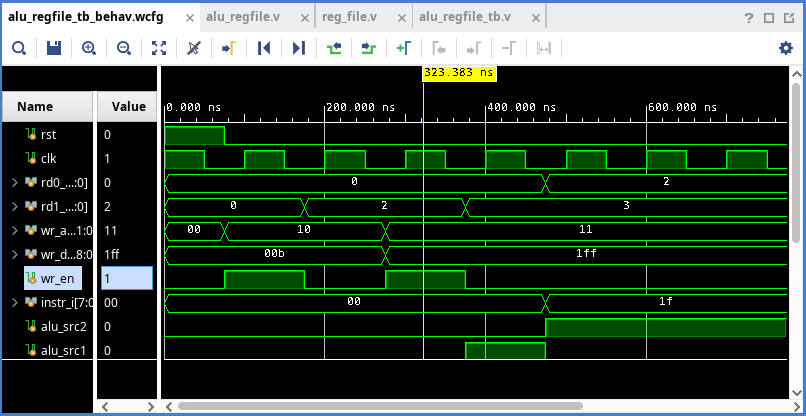
\includegraphics[width=\linewidth]{image}
	\caption{Test bench output}
\end{figure}

\begin{lstlisting}
module alu_regfile_tb();

    reg rst;
    reg clk;
    reg [1:0]rd0_addr;
    reg [1:0]rd1_addr;
    reg [1:0]wr_addr;
    reg [8:0]wr_data;
    reg wr_en;
    reg [7:0]instr_i;
    reg alu_src2;
    reg alu_src1;
    reg [2:0]alu_op;
    wire [7:0]result;
    wire [7:0]input1;
    wire [7:0]input2;
    wire ovf;
    wire take_branch;

    alu_regfile sdlkf(
        .rst(rst),
        .clk(clk),
        .rd0_addr(rd0_addr),
        .rd1_addr(rd1_addr),
        .wr_addr(wr_addr),
        .wr_data(wr_data),
        .wr_en(wr_en),
        .instr_i(instr_i),
        .alu_src2(alu_src2),
        .alu_src1(alu_src1),
        .alu_op(alu_op),
        .result(result),
        .input1(input1),
        .input2(input2),
        .ovf(ovf),
        .take_branch(take_branch)
    );

    initial begin
        clk = 1;
        forever begin
            #50; 
            clk = ~clk;
        end
    end

    initial begin
        rst = 1;
        rd0_addr = 0;
        rd1_addr = 0;
        wr_addr = 0;
        wr_data = 11;
        wr_en = 0;
        instr_i = 0;
        alu_src2 = 0;
        alu_src1 = 0;
        alu_op = 0;

    #25;

    #50;

    rst = 0;
    wr_addr = 2;
    wr_en = 1;

    #100;

    wr_en = 0;
    rd1_addr = 2;    

    #100;

    wr_en = 1;
    wr_addr = 3;
    wr_data = 511;

    #100;

    wr_en = 0;
    alu_op = 3;
    rd1_addr = 3;
    alu_src1 = 1;

    #100;

    instr_i = 31;
    alu_op = 2;
    alu_src1 = 0;
    rd0_addr = 2;
    alu_src2 = 1;

    end
endmodule
\end{lstlisting}

\subsection*{Lab 5}

\begin{figure}
	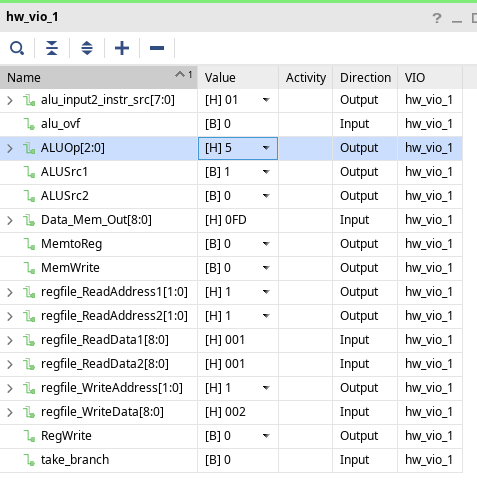
\includegraphics{image2}
	\caption{Here we have the sll step, and we also see that the expected
	value is stored in the Data Memory location (stored earlier).}
\end{figure}


\end{document}
